\documentclass[border=10pt]{standalone}
\usepackage{tikz}
\usetikzlibrary{arrows.meta, shapes, calc, positioning}

\begin{document}
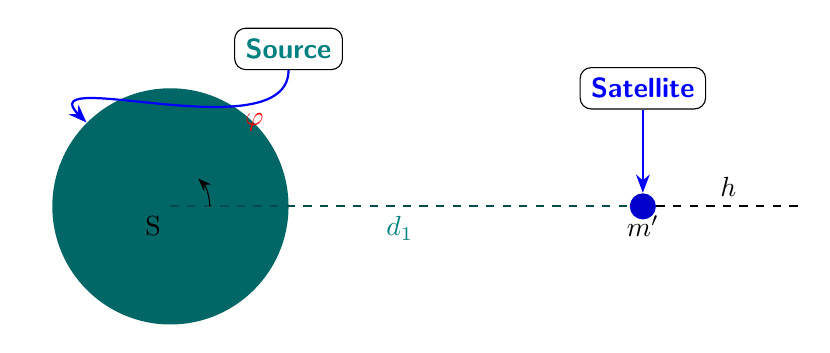
\begin{tikzpicture}[
    source/.style={fill=teal!80!black, circle, minimum size=3cm},
    satellite/.style={fill=blue!80!black, circle, minimum size=4pt},
    labelbox/.style={draw, rounded corners, font=\sffamily\bfseries, inner sep=4pt},
    arrow/.style={->, >=Stealth, thick, blue}
]

% Source circle
\node[source] (source) at (0,0) {};
\node at (source.center) [below left] {S};

% Phi symbol near surface
\node[red] at (source.45) {$\varphi$};

% Satellite point
\node[satellite] (satellite) at (6,0) {};
\node[below] at (satellite) {$m'$};

% Distance d1
\draw[dashed, thick, teal!60!black] (source.center) -- (satellite) node[midway, below, teal] {$d_1$};

% Direction h
\draw[dashed, thick] (satellite) -- ++(2,0) node[midway, above] {$h$};

% Source label
\node[labelbox, text=teal] (source_label) at (1.5,2) {Source};
\draw[arrow] (source_label) to[out=-90, in=135] (source.135);

% Satellite label
\node[labelbox, text=blue] (satellite_label) at (6,1.5) {Satellite};
\draw[arrow] (satellite_label) to[out=-90, in=90] (satellite);

% Curved arrow from center to surface
\draw[->, >=Stealth, thin, black] (source.center) ++(0.5,0) arc (0:45:0.5);

\end{tikzpicture}
\end{document}